\documentclass{article}
\usepackage[utf8]{inputenc}
\usepackage{amsmath,amssymb,bm}
\usepackage{mathtools}
\usepackage{graphicx,caption}
\usepackage{listings}
\usepackage[margin=1.2in]{geometry}

\usepackage{titling}
\usepackage{lipsum}

\usepackage{parskip}

\usepackage{url}

\usepackage[
    style=authoryear-icomp,
    maxbibnames=9,
    maxcitenames=2,
    backend=biber
]{biblatex}
\addbibresource{sample.bib}

\setlength{\jot}{10pt}

\allowdisplaybreaks[1]

% Expectation symbol
\DeclareMathOperator*{\E}{\mathbb{E}}

% Math functions
\DeclareMathOperator{\Span}{span}

% Conditional
\newcommand\given[1][]{\:#1\vert\:}

% argmax
\DeclareMathOperator*{\argmax}{arg\,max}
\DeclareMathOperator*{\softmax}{soft\,max}

\graphicspath{{images/}}

\title{%
    Adversarial Text Generation\\
    \large NLP and Deep Learning --- Final Project\\
    \small KSNLPDL2KU
}

\author{%
    Andreas Holck Høeg-Petersen\\
    \texttt{anhh@itu.dk}
    \and
    Mathias Bastholm\\
    \texttt{mbas@itu.dk}
}

\begin{document}
\maketitle

\section{Introduction}\label{sec:introduction}

In recent years, Generative Adversarial Networks (GANs) have gained a lot of
traction in the Deep Learning community because of their impressive results in
image generation. The general idea is that a generator and a discriminator are
jointly trained to produce an image output that is seemingly indistinguishable
from non-generated images. This model were first described
in~\cite{Goodfellow2014GenerativeAN}.

We want to attempt to apply this strategy for text generation. The main
difficulty for this task is that whereas image outputs can be considered a
continuous value, a sentence is inherently discrete as it is a sequence of words
each of which is chosen by the model using the non-differentiable $argmax$
function. To remedy this, we propose a model where the discriminator is trained
to distinguish between the continuous outputs of a pre-trained encoder given a
`true' sentence from the generated, `fake' output stemming from our generator.

\begin{figure}[h]
    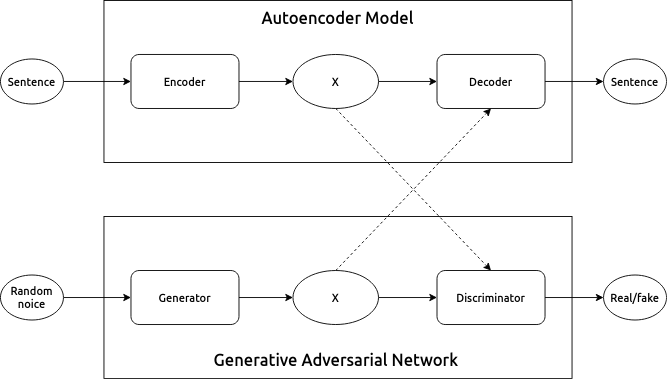
\includegraphics[width=\textwidth]{projectModel.png}
    \caption{% 
        Overview of the model architecture. The dotted lines from the
        $\mathbf{X}$s represents that the encoded and generated $\mathbf{X}$s
        will be fed to the discriminator and the decoder during training and
        evaluation, respectively.
    }\label{fig:projectModel}
\end{figure}

In our project, we will construct and train an autoencoder model that can encode
and decode a sentence from English to English. The encoded sentences are then
used as labelled training data for the discriminator, representing `true'
values. The job of the generator is to produce similar encodings but doing this
from random noise in a way that makes the discriminator unable to distinguish
between the encodings stemming from the autoencoder and the encodings stemming
from the generator.

Ideally, this would train the generator to produce sentence encodings that can
be fed to the decoder of the Transformer model which would then produce
meaningful sentences from this artificially generated input. See
Figure~\ref{fig:projectModel} for an overview of the complete model.

This project thus have two objectives: one is to construct a working autoencoder
that can map an English sentence to some hidden state $\mathbf{X}$ with a
corresponding decoder that can extract the original sentence from $\mathbf{X}$.
For convenience, we will refer to the encoder part of this model as the
`Teacher'. The second objective is to build a GAN network, where a generator ---
the `Student' --- must learn to produce approximations of $\mathbf{X}$.

The second objective is highly experimental as explained in
Section~\ref{sec:background}, where we will also describe other approaches at
using the GAN architecture for NLP problems.  We will then describe how we have
build the different parts of the model and how we utilize our dataset.  Then we
will present our results and discuss the shortcomings of the model\(s\), and
proceed to suggest improvements and ideas for further research.  Lastly we
provide a conclusion on the project.

The entire source code for the project is available at the GitHub repository for
the project:
\url{https://github.com/andreashhpetersen/adversarial-text-generation}


\section{Background}\label{sec:background}

Applications GANs have mainly focused on image generation and has not yet seen a
major breakthrough in text generation. As mentioned in
Section~\ref{sec:introduction}, this is because the discrete nature of text,
which is basically a sequence of words, requires a non-differentiable $argmax$
function to transform a probability distribution over a vocabulary to a single
value (ie.\ the word with the highest probability). This is depicted in
Figure~\ref{fig:argmaxGAN}.

\begin{figure}[h]
    \centering
    \captionsetup{width=0.8\textwidth}
    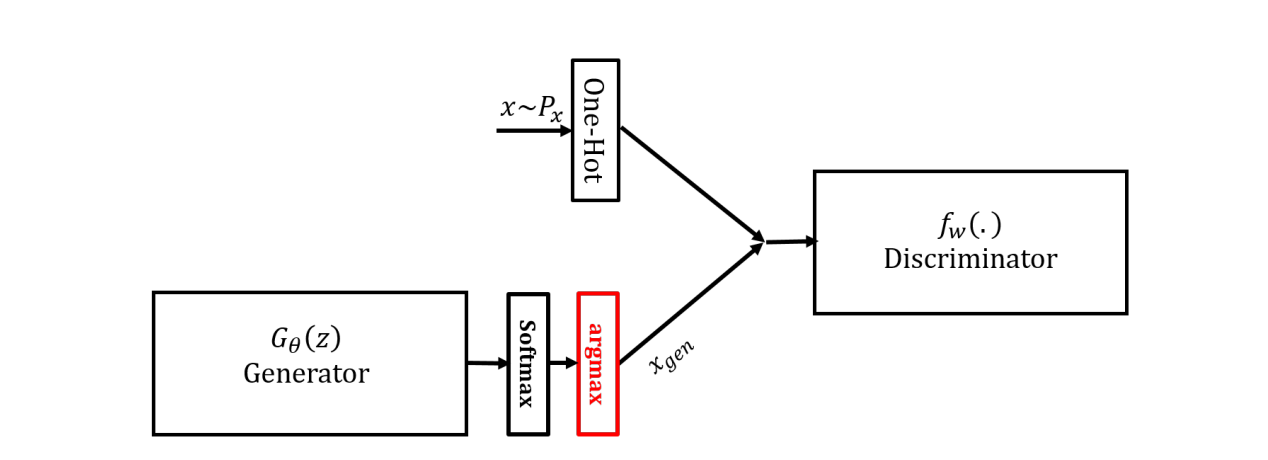
\includegraphics[width=0.8\textwidth]{argmaxGAN.png}
    \caption{%
        A simple GAN model where the generator output is run through an
        $argmax$ function before being given to the discriminator. This prevents
        gradients to flow from the discriminator to the generator.
        Source:~\cite{haidar2019textkdgan}.
    }\label{fig:argmaxGAN}
\end{figure}

There have been, however, multiple attempts at working around this issue.
According to~\cite{Chintapalli2019} these approaches can broadly be categorized
into three types:

\begin{itemize}
    \item Reinforcement Learning-based solutions
    \item The Gumbel-Softmax approximations
    \item Avoiding discrete spaces by working with the continuous output of the
        generaor
\end{itemize}

In this project, we follow the third approach, but in this section we will give
short introductions to the idea behind the two first.

As an example of an RL-based solution,~\cite{yu2016seqgan} proposes the SeqGAN
model, in which the generator is considered an RL-agent with states
$\mathbf{s}_t$ being the text generated at timestep $t$ and actions $\mathbf{a}$
being all the possible words to choose next. The agent then chooses its next
word (takes an action $a$) based on some policy function $\bm{\pi}(a \given
\bm{s}_t, \bm{\theta})$, where $\bm{\theta}$ are the parameters to be
optimized. Using Monte-Carlo rollouts to produce a number of different
sentences sharing a prefix $\bm{s}_t$, the discriminator then rewards each
sentence and the averaged reward is then used to perform gradient ascent on
$\bm{J}(\bm{\theta})$, where $\bm{J}$ is the performance measure of
$\bm{\theta}$. This approach alleviates some of the problems of training a GAN
for text generation, but it suffers from an unstable and slow training process,
convergence to sub-optimal local minima and and extremely large state-space.\

Another approach is to use the Gumbel-Softmax distribution to approximate a
one-hot encoding of a probability distribution passed through the $argmax$
function. This is the approach taken by~\cite{kusner2016gans}. Here, a
$d$-dimensional one-hot encoding vector $\bm{y}$ is approximated using

\begin{equation}
    \bm{y} = \softmax(\frac{1}{\tau}(\bm{h}+\bm{g}))
\end{equation}

where $\bm{h}$ is some hidden state (ie.\ of an RNN), $\bm{g}$ is drawn from a
Gumbel distribution and $\tau$ is a temperature parameter. This works because it
is differentiable and as $\tau \to 0$ the distribution of $\bm{y}$ will match
that we get from

\begin{equation}
    \bm{y} = \text{one\_hot}(\argmax_{i}(h_i + g_i))
\end{equation}

which again can be shown to be the same as sample $\bm{y}$ from a probability
distribution $\bm{p} = softmax(\bm{h})$ where $p_i = p(y_i=1), i = 1\dots d$.

Finally, for other examples on the third approach,
see~\cite{donahue2018adversarial} and~\cite{haidar2019textkdgan}.


\section{Method}\label{sec:method}

For all our models (autoencoders and GANs), we drew inspiration PyTorch
tutorials
(\cite{pytorchTutorialAtt}, \cite{pytorchTutorialTransformer}, \cite{pytorchTutorialGAN}),
tweaking them to our specific needs. The whole process (project development,
research, data collection, coding, training, experimentation and analysis) was
conducted during a 10-day period.

This section will describe this process, focusing on the final outcomes rather
than including all our intermediate steps and missteps.

\subsection{Dataset}\label{sec:dataset}

For training of the autoencoders, we simply needed dataset consisting of a large
number of English sentences. We obtained this from Universal Dependencies, where
used the `Universal Dependencies --- English Dependency Treebank Universal
Dependencies English Web Treebank v2.6 --- 2020--05--15' (\cite{silveira14gold})
consisting of 12,543 training sentences, 2,077 test sentences, 2,002 dev
sentences and a vocabulary of 16,654 training tokens. The data is annotated with
metadata such as lemmas and word classes, but we discarded this information as
it was not relevant for our purpose.

Furthermore, we also utilized another dataset intended for training
English-to-French translation. This dataset originates from
\url{https://tatoeba.org/eng/} and consists of 135,842 sentence pairs. We
discarded the French sentences and removed all duplicate sentences and sentences
of length smaller than 3, as well as splitting all sentences that contained
punctuations, questionmarks, exclamation points, etc. This gave us a set of
92,343 sentences, which we split 80/10/10 between training and training/validation/testing.
 The dataset had a vocabulary of 13,731 tokens.


\subsection{Models}\label{sec:models}

We developed two different versions of the autoencoder model and one GAN model.
These will be described in this subsection.

\subsubsection{The TransformerModel}\label{sec:transformermodel}

Our first autoencoder was based on~\cite{pytorchTutorialTransformer}. This model
consists of a very simple decoder, that is simply a feed-forward neural net that
takes a 2-dimensional tensor $X \in \mathbb{R}^{n \times k}$ and maps each of
the $n$ $k$-dimensional vectors of the sequence to a probability distribution
over the entire vocabulary which it then can convert to an output sequence using
$argmax$.

The encoder, however, is responsible for generating $X$ and it does so by using
the Transformer architecture as suggested in~\cite{vaswani2017attention} and
implemented in the PyTorch module \texttt{nn.Transformer}. For our purpose,
however, we only used the submodule \texttt{nn.TransformerEncoder}, which
consists of a stack of encoder layers that uses self-attention to focus on
specific, relevant parts of the input sequence in one go, and then passes its
output on to the next layer through a feed-forward network. As a preprocessing
step, before the input sequence is passed through the transformer, positional
encoding is added, as suggested in the paper (\cite{vaswani2017attention}).

This model also uses an embedding as its first layer. For embeddings, we use
pretrained word vectors from the \texttt{polyglot} Python package. These have an
embedding size of 64, which therefore what we use across all models. Note that
the next, RNN-based autoencoder uses the same embedding setup.


\subsubsection{RNN and Attention based Autoencoder}\label{sec:attnRNN}

In our second model, the heavy-lifting is switched from the encoder to the
decoder. Again, we utilize the attention mechanism, but this time it is combined
with an RNN architecture, more precisely a Gated Recurrent Unit (GRU). In this
model, the encoder is simply a GRU layer that processes the entire sequence and
then its final hidden state aswell as the output for each word in the sequence
is passed to the decoder.

The decoder has a bit more to it. On each timestep it takes in its own last
output (starting with the special \texttt{start-of-sequence}-token), a hidden
state (starting with the last hidden state of the encoder) and all the encoder
outputs. It then uses a linear layer (ie.\ a simple feed-forward network) to
calculate the attention weights by combining the input and the current hidden
state. The attention weights and the encoder outputs are then mulitplied
together using matrix multiplication and the result of this operation can then be
merged with the original input and passed through another linear layer to
produce a vector of size \texttt{(sequence\_length * hidden\_size)}.

In this vector, the decoder has now embedded all the information about where to
focus its attention, and it can pass this to a GRU just as in the encoder ---
however, opposite to the GRU in the encoder, the output of the recurrent layer
in the decoder is responsible for mapping back to actual words. This mapping is
finalized by an output linear layer that expands the hidden size to the size of
the vocabulary and then, finally, a $softmax$ operation converts the output to
probability distributions.

When the decoder outputs the special \texttt{end-of-sequence}-token it is
finished and the process terminates. Our implementation of this model is based
on~\cite{pytorchTutorialAtt}.


\subsubsection{GAN}\label{sec:modelGAN}

Our GAN model is modelled after our TransformerModel in an attempt to mimic the
inner mechanics of the network it is trying to imitate. As stated, a GAN
consists of a generator and a discriminator. The generator gets a vector of
random noise as input. This vector has dimensions \texttt{(max\_sequence\_length
* embedding\_size)}. The reason we set a parameter
\texttt{max\_sequence\_length} is because neural networks expects static sizes,
but since sentences can have different lengths, we set an upper bound. The
generator should, however, be able to encode its output in a way, that produces
sentences of length 0 to \texttt{max\_sequence\_length} (ie.\ by encoding an
\texttt{end-of-sequence}-token at some position).

The generator passes its input through a linear layer and then, as the
TransformerModel, adds positional encoding before it runs it through an encoder
stack (\texttt{nn.TransformerEncoder}). The final output has the same shape as
the output of the encoder part of the TransformerModel.

The discriminator has almost the same structure as the generator (it uses
positional encoding and an encoder stack), but the input differs and it outputs
a single number between 0 and 1. Recall, that the job of the discriminator is to
decide wether its input was generated from random noise via the generator or if
it was an encoding stemming from a real sentence passed through a trained
encoder. Thus, it is effectively a binary classifier, and its output should
describe its conviction that the input is `true'.

\subsection{Training}\label{sec:training}

Our training had two aspects: first, we had to train our autoencoders on
English-to-English sentence pairs, and then we had to train our GAN model. This
section will describe both.

\subsubsection{Training the autoencoders}\label{sec:trainingAutoEnc}

This part is pretty straight forward. We give the model a batch of sentences
which it then encodes and decodes again. Since the input sentence is also the
target sentence, the loss is simply the difference between the input and the
output. To calculate this loss, we use PyTorchs `nn.CrossEntropyLoss' which
takes the raw output of the model (ie.\ before it has been converted to a
probability distribution) and a target vector and then calculates the negative
log-likelihood loss. We use Stochastic Gradient Descent to update the weights of
the models.

There were some notable differences between the way we trained the
TransformerModel and the RNN-based model. For the TransformerModel we had good
results with a learning rate of 0.05, and we performed training on the entire
training set in batches of 8 and over the course of 25 epochs. We also trained
it another time with just 5 epochs, but this time without ignoring the padding
in the batches (when batching the data, not all sentences have the same length
and the smaller sentences are padded with the special \texttt{<PAD>}-token).
This makes the model achieve a lower loss much faster, as it quickly learns the
pattern of the padding tokens, but this often comes at the expense of the model
learning the actual sentence, which generally is what is of interest. However,
we wanted our Student model to learn both from a Teacher that had learned
padding and one that hadn't, so we trained the autoencoders (Teacher) on both.

In training the RNN-based model we took inspiration
from~\cite{pytorchTutorialAtt}. This means we set the learning rate to 0.01 and
instead of training on the entire training set over multiple epochs, we let the
model randomly pick a data batch, train on that and then pick a new for 60,000
iterations. Furthermore, we used teacher forcing, where instead of letting the
output of the decoder be its own next input, we give the actual next input (from
the target sentence). This approach can lead to some terrible cases of
overfitting and preventing the model form learning its mistakes properly, but in
the right dose it can also help the model converge faster. Therefore, for each
training instance, we chose with 50\% probability wether to use teacher forcing
or not.


\subsubsection{Training the GAN model}\label{sec:trainingGAN}

The training of the GAN model is the interesting and difficult process. Here, we
have to simultaneously train two different models that work towards opposite
goals. One, the generator, will have to learn how to maximise the probability
that the discriminator classifies its output as `true', while the other, the
discriminator, will have to learn to maximise the probability that it classifies
the output of the generator as `fake' while also classifying the output of the
Teacher (encoder) as `true'. So the two components engage in a min-max game
with one another.

Formally, let $G$ and $D$ be the generator and the discriminator respectively
and let $x$ be the data representing a sentence (encoded or generated). Then,
$D(x)$ is the output of the discriminator given some data, and we want this to
be high when $x$ is `true' (stemming from the Teacher) and low when $x$ is
`fake' (generated by the Student). Let $z$ be some random noise, and then we
have that $G(z)$ is the output generated by the Student given some random noise.
So, the discriminator now tries to \textit{maximize} the probability that it
correctly classifies `true' and `fake' data, $\log D(x)$, and the generator
tries to \textit{minimize} the probability that the discriminator classifies its
outputs as `fake', $\log(1 - D(G(z)))$. As described in the original GAN
paper~\cite{Goodfellow2014GenerativeAN}, this can be formalised as:

\[
    \min_G \max_D V(D,G) = {\E}_{x \sim p_{data}(x)}\left[\log D(x)\right] +
        {\E}_{z \sim p_{z}(x)}\left[\log(1 - D(G(z)))\right]
\] 

where $p_{data}$ is the `true' distribution over the real data which the
generator tries to estimate, and $p_z$ is the estimated distribution that the
generator draws its samples from.

The way we do this is by following the approach suggested
by~\cite{Goodfellow2014GenerativeAN} and PyTorch GAN tutorial for image
generation~\cite{pytorchTutorialGAN}. This involves first giving the
discriminator a batch of `real' input (ie.\ input generated by the Teacher) and
then calculating the loss and the gradients based on its performance. Then we
give it a batch of `fake' data generated by the Student, again calculating the
loss and gradients. Then, before we move on to training the generator, we
perform our optimization step for the discriminator. When we then pass the
output of the generator through the discriminator, the discriminator has been
updated and the generator will have to learn to adjust to this. 

However, one could imagine that the generator could learn to just output random
words very well and that the discriminator would not be able to distinguish this
from a `real' sentence. Therefore, before training the generator, we also give
the discriminator a batch of `fake' data that has been generated by the encoder,
but when the encoder have gotten random words as input. This, in theory, should
force the generator to produce meaningful sentences (not just random words) for
it to be classified as `true' by the discriminator. This adjustment is specific to
our approach.

It is worth noting, that training a GAN is known to be highly non-trivial
(\cite{Hui2018}) and even small variations in the hyperparameters, number of training
iterations or internal structure of the generator and/or discriminator can make
the model collapse spectacularly.

\section{Results and analysis}\label{sec:analysis}

In this section, we will present and discuss our results as well as give
suggestions for further improvements and research.

\subsection{TransformerModel}

As stated, we trained the TransformerModel both with and without ignoring
padding. Generally, we achieved nice results here, with a word accuracy around
99\%. In Figure~\ref{fig:transformerLossNoPadding}
and~\ref{fig:transformerLossPaddingEOS} we have plotted the loss.

\begin{figure}[h]
    \centering
    \begin{minipage}{0.45\textwidth}
        \captionsetup{width=0.8\textwidth}
        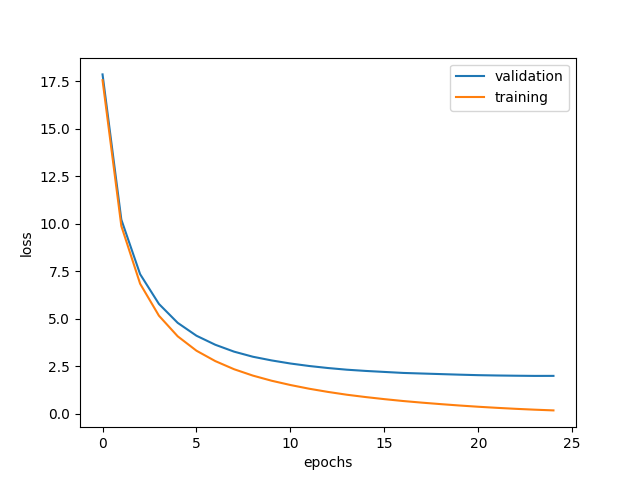
\includegraphics[width=0.9\textwidth]{transformer.png}
        \caption{%
            Loss of the standard TransformerModel
        }\label{fig:transformerLossNoPadding}
    \end{minipage}
    \begin{minipage}{0.45\textwidth}
        \captionsetup{width=0.8\textwidth}
        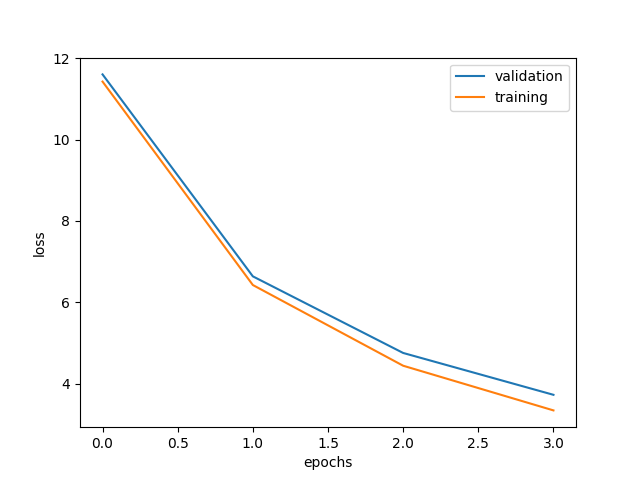
\includegraphics[width=0.9\textwidth]{transformer_padding-eos.png}
        \caption{%
            Loss of the TransformerModel that takes padding into account and has
            EOS tokens. Even with way fewer epochs, the results were very good.
        }\label{fig:transformerLossPaddingEOS}
    \end{minipage}
\end{figure}


The following are some examples of how the model performed on specific inputs:

\begin{verbatim}
++++++ Successful encoding ++++++
> he can play the piano , the flute , the guitar , and so on .
< he can play the piano , the flute , the guitar , and so on .

> i have to take the entrance examination today .
< i have to take the entrance examination today .

++++++ Failed encoding ++++++
> i'm sure it wouldn't be too hard to find out who hacked into our system .
< i'm sure it wouldn't be too hard to find out who weakly into our system .

> you have the right to free speech , but not the right to slander .
< you have the right to free speech , but not the right to limits .
\end{verbatim}

And here are some examples of the model when train with padding and
\texttt{end-of-sequence}-token:

\begin{verbatim}
> his house was small and old . <EOS>
< his house was small and old . <EOS>

> i realized what was happening . <EOS> <PAD>
< i realized what was happening . <EOS> <PAD>

> there is no museum . <EOS> <PAD> <PAD> <PAD>
< there is no antidote . <EOS> <PAD> <PAD> <PAD>
\end{verbatim}

Notice the error in the last sentence. For good measure, we report the following
input/output-pair that was observed during training. Maybe the model were
developing a political opinion, maybe it was joking. We will probably never
know:

\begin{verbatim}
> rwandan rebels are pushing their offensive south as fighting continues in the capital kigali . <EOS>
< honest guys are noticed their interesting south as fighting awake in the capital fortune . <EOS>
\end{verbatim}

\subsection{RNNModel}

Our RNN-based model performed much worse, than we had expected. It also took an
extraordinary amount of time to train, so we only did so many experiments. A
plot of the loss can be seen in Figure~\ref{fig:rnnLoss}. 

\begin{figure}[h!]
    \captionsetup{width=0.8\textwidth}
    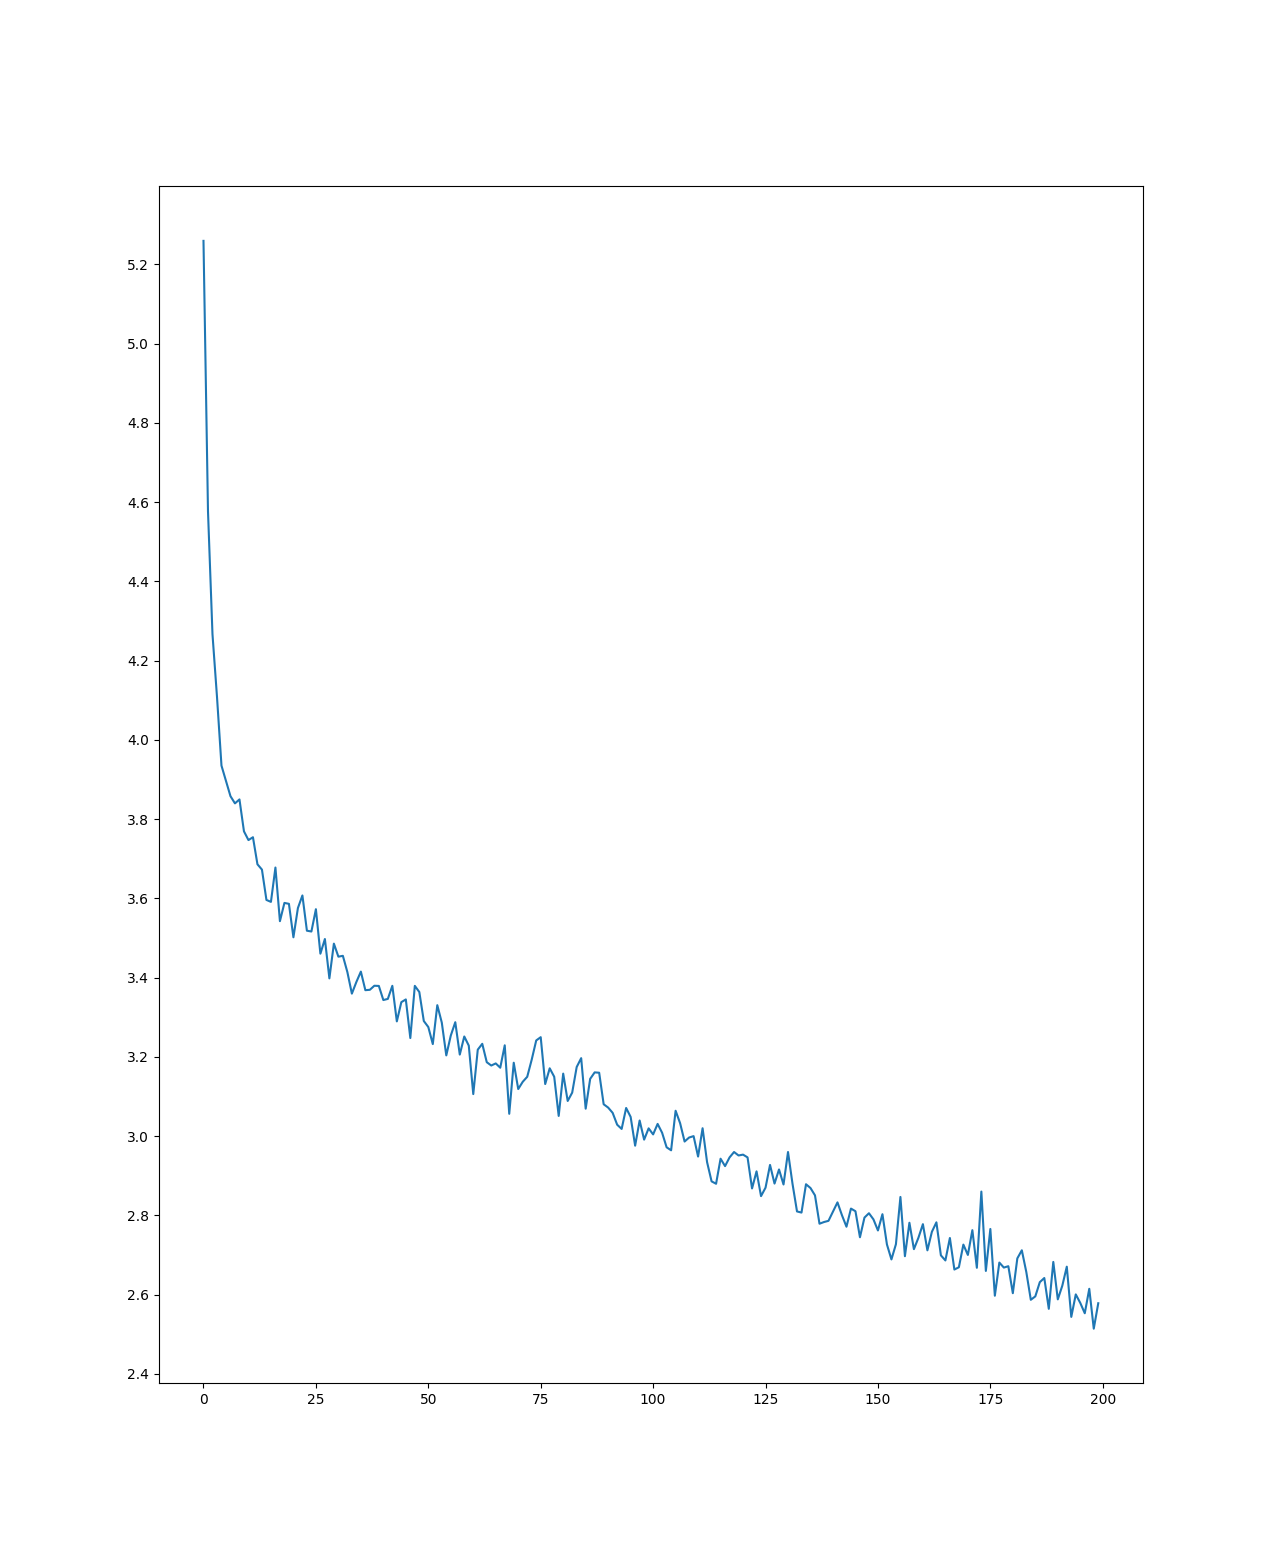
\includegraphics[width=0.9\textwidth, height=15cm]{RNN-loss-part1.png}
    \caption{%
        Training loss of RNN-based attention model.
    }\label{fig:rnnLoss}
\end{figure}

We trained the same model several times with decreasing batch size, and even
though the loss kept going down, the following examples show that the end result
was not amazing:

\begin{verbatim}
> tom got to the station too late so he missed the train . <EOS> <PAD>
< tom got to the so so so he opened the same . <EOS>

> i don't want to waste my time trying to do this again . <EOS> <PAD>
< i don't want to take my job to do me it . <EOS>

> if the car is gone , he can't be at the office . <EOS> <PAD>
< if the book is he , he was late than the . <EOS>

> i can't believe that you were the smartest kid in your class . <EOS> <PAD>
< i can't believe that you were a a the in the . . <EOS>
\end{verbatim}

It has clearly learned something, most notably \texttt{end-of-sequence}-tokens
and padding. Further, it seems that it does a fine job in the beginning of
sentences, but then looses track of what to do. This indicates that it hasn't
picked up on long-term dependencies in the sentences, which might could be
alleviated with another RNN-unit (eg.\ an LSTM) or more training.

\subsection{GAN}

Now, lets look at the results of our GAN model. Because of the poor performance
of out RNN-based autoencoder and some technical difficulties, we only trained the
GAN against the TransformerModel. Also, we set the maximum sequence length to be
10 which is fine for prototyping and evaluating if anything is actually learned.

Beginning with Figure~\ref{fig:ganLossAdam} and Figure~\ref{fig:ganLossSGD} we
see how the networked performed when trained with Adam and Stochastic Gradient
Descent respectively as its training algorithm. The difference is very clear:
for Adam, the generator and the discriminator has a pretty consistent
relationsship until suddenly, the discriminator seem to figure out how to call
bluff on the generator, and the generator has no answer to that. The loss goes
way up for the generator and it falls to a minimum for the discriminator and the
model seem to collapse.

For SGD, the model is in some sense way more stable and the loss for both the
discriminator and the generator stays in same limited interval. 

\begin{figure}[ht]
    \begin{minipage}{0.45\textwidth}
        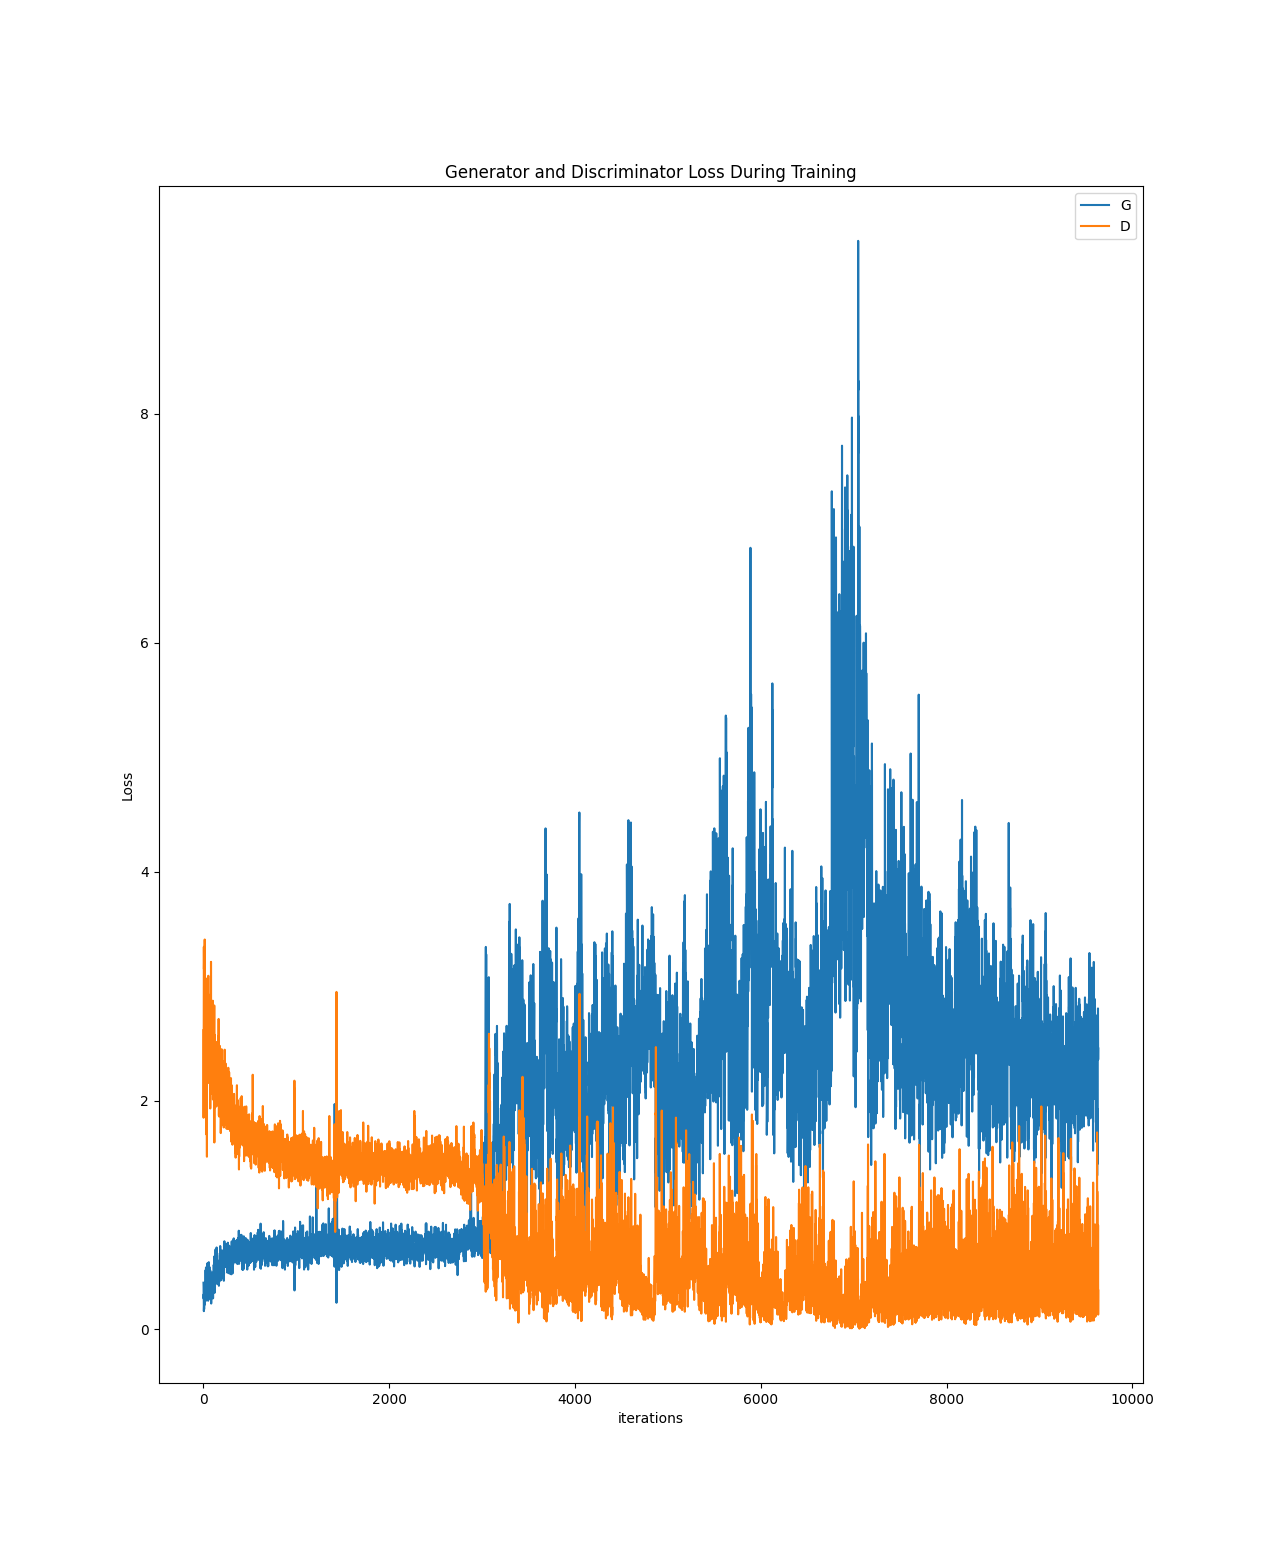
\includegraphics[width=\textwidth, height=5cm]{GAN-loss-Adam.png}
        \caption{%
            GAN loss using Adam
        }\label{fig:ganLossAdam}
    \end{minipage}
    \begin{minipage}{0.45\textwidth}
        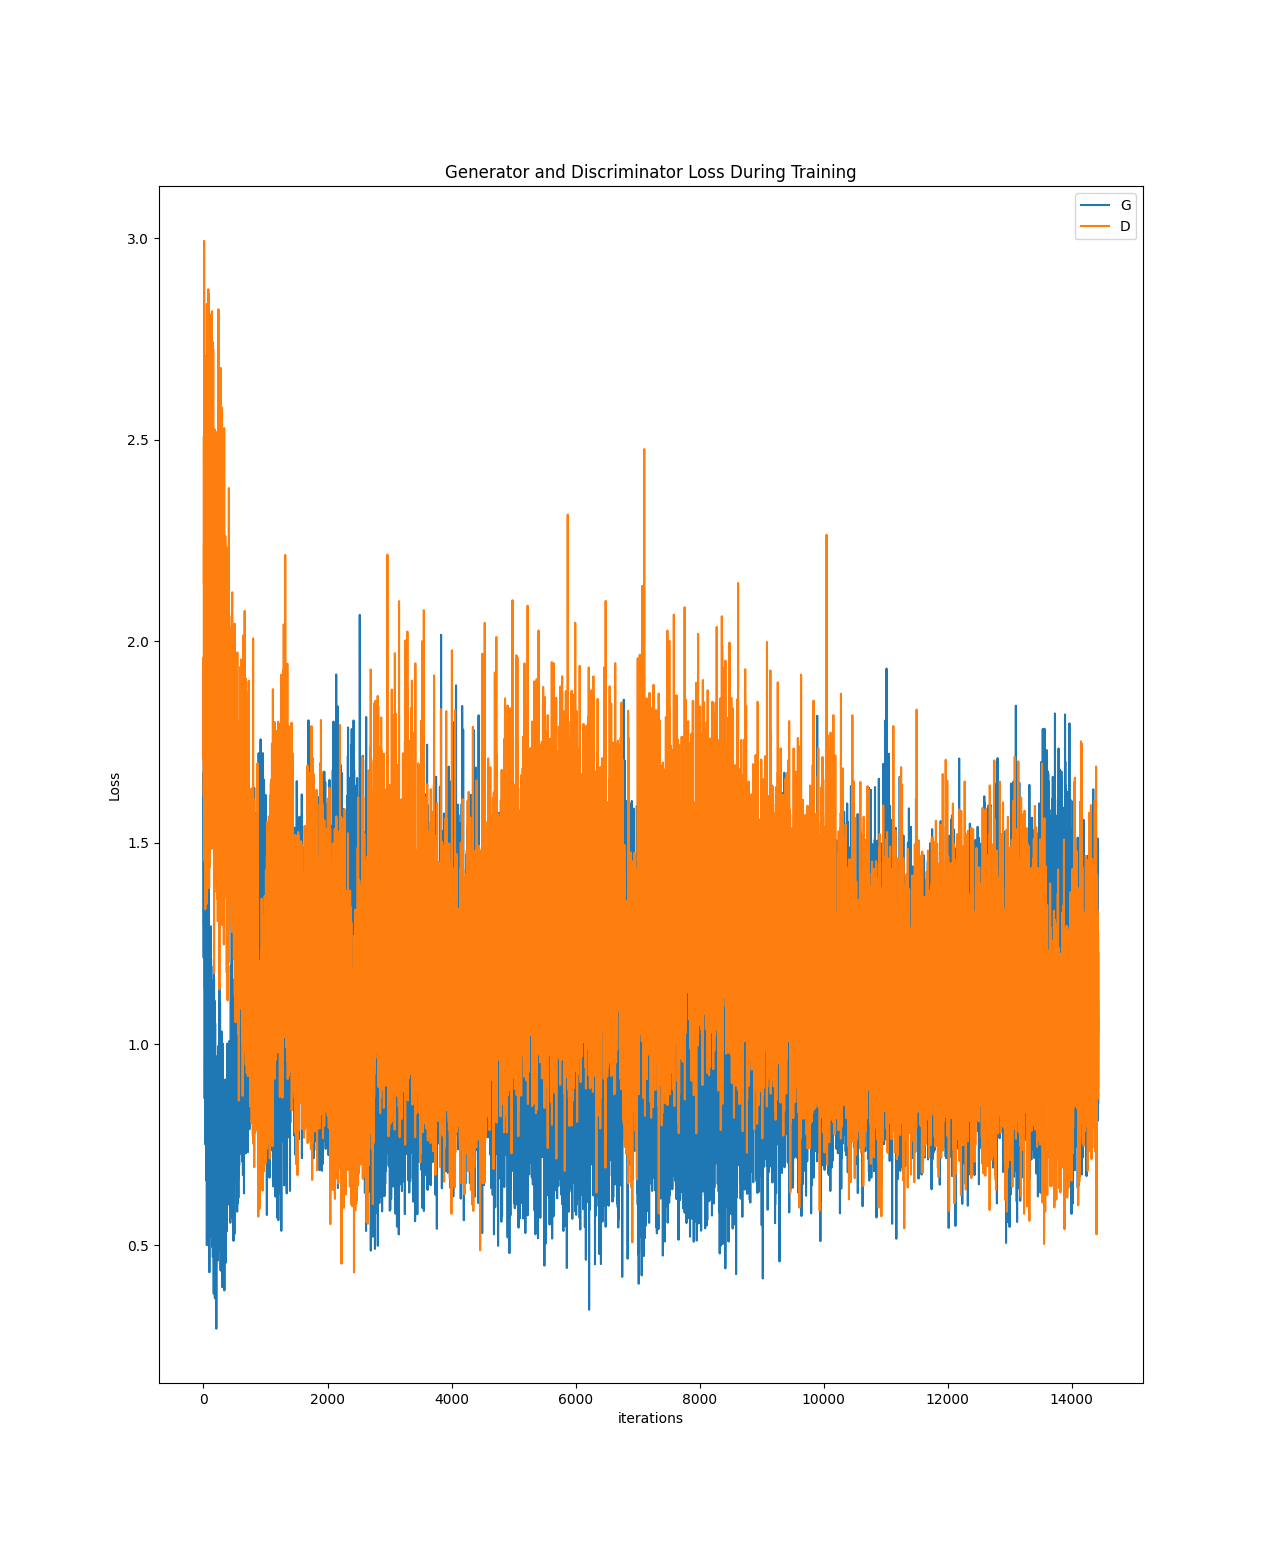
\includegraphics[width=\textwidth, height=5cm]{GAN-loss-SGD.png}
        \caption{%
            GAN loss using SGD
        }\label{fig:ganLossSGD}
    \end{minipage}
\end{figure}

Since what we really wanted was a strong generator, and this seemed to be the
component that failed, we tried training with a double batch for the generator
to give an edge against the discriminator. The resulting loss is seen in
Figure~\ref{fig:ganLossAdamDoubleBatch} and
Figure~\ref{fig:ganLossSGDDoubleBatch}. The pattern is the same, but this time,
the Adam model collapses faster.

\begin{figure}[ht]
    \begin{minipage}{0.45\textwidth}
        \captionsetup{width=0.8\textwidth}
        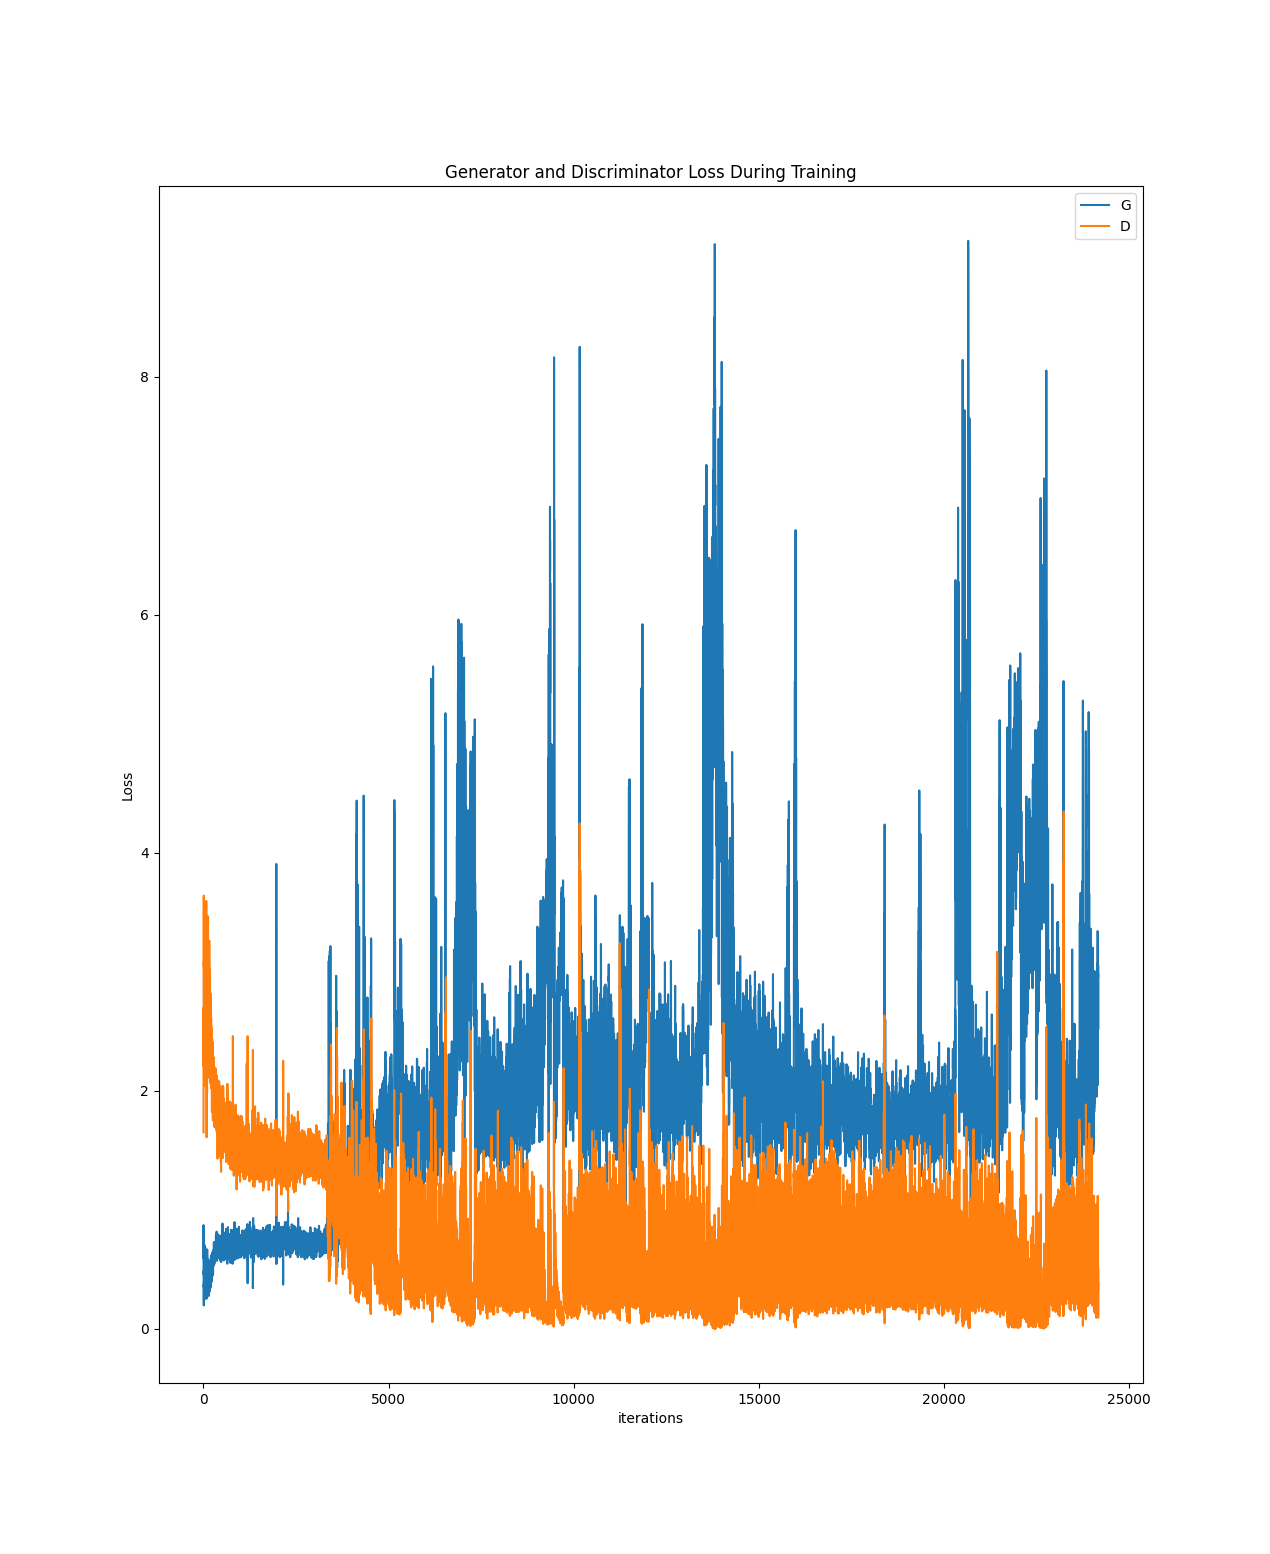
\includegraphics[width=\textwidth, height=5cm]{GAN-loss-double_batch-Adam.png}
        \caption{%
            GAN loss using Adam and double batch for generator
        }\label{fig:ganLossAdamDoubleBatch}
    \end{minipage}
    \begin{minipage}{0.45\textwidth}
        \captionsetup{width=0.8\textwidth}
        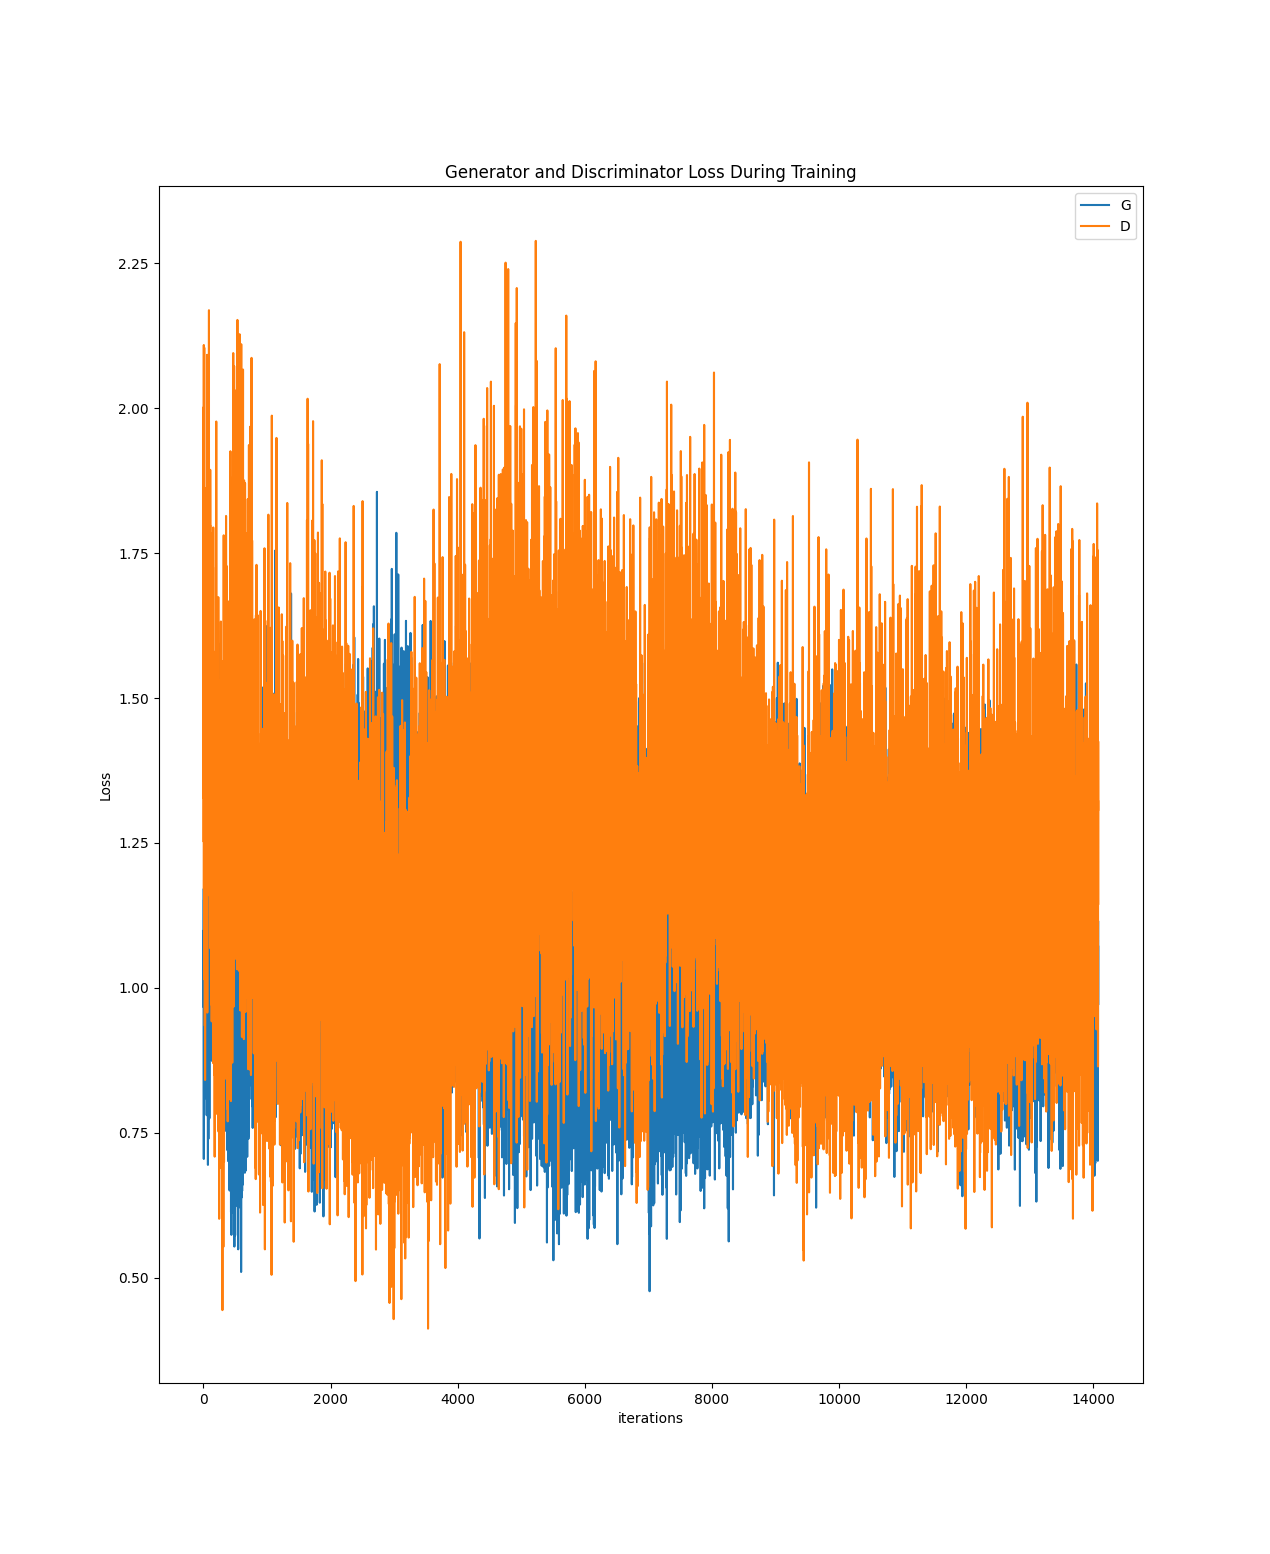
\includegraphics[width=\textwidth, height=5cm]{GAN-loss-double_batch-SGD.png}
        \caption{%
            GAN loss using SGD and double batch for generator
        }\label{fig:ganLossSGDDoubleBatch}
    \end{minipage}
\end{figure}

Looking at the actual output, we some interesting results. First, lets look at
some output from the Adam training (without double batch):

\begin{verbatim}
[0/10][0/6765]      Loss_D: 1.8526  Loss_G: 0.6623  D(x): 0.5776    D(G(z)): 0.5878 / 0.5499
know for know i'm i'm the for good some i'm

[0/10][500/6765]    Loss_D: 1.7199  Loss_G: 0.6846  D(x): 0.2188    D(G(z)): 0.5105 / 0.5054
your appropriated make ? but <PAD> <EOS> <EOS> <PAD> <PAD>

[0/10][2000/6765]   Loss_D: 1.2057  Loss_G: 0.9821  D(x): 0.2932    D(G(z)): 0.4748 / 0.3959
your out out out out out <EOS> <EOS> <PAD> <PAD>

...

[2/10][2450/6765]       Loss_D: 1.4581  Loss_G: 1.7943  D(x): 0.2807    D(G(z)): 0.1915 / 0.1928
tom cats a a stayed . <EOS> <PAD> <PAD> <PAD>

[2/10][2950/6765]       Loss_D: 0.4975  Loss_G: 1.7132  D(x): 0.3910    D(G(z)): 0.0857 / 0.2305
he who painted is is . <EOS> <PAD> <PAD> <PAD>

[2/10][3450/6765]       Loss_D: 0.4640  Loss_G: 6.3138  D(x): 0.3933    D(G(z)): 0.1249 / 0.0479
don't child caught more my . . <EOS> <PAD> <PAD>
\end{verbatim}

These are outputs that show, what the loss of the discriminator (Loss\_D), the
loss of the generator (Loss\_G), the average discriminator output on
non-generated data ($D(x)$) and the average discriminator output on the
generated data before and after updating the discriminator ($D(G(z))$).

When we train the discriminator on encoded random words, $D(x)$ should be 0.5
for a perfect $D$ (because half of $x$ is `true' and the other half is `fake').
When omitting the encoded random words, $D(x)$ should be 1. Of course, for a
perfect network with a perfect $D$ and a perfect $G$, both $D(x)$ and $D(G(z))$
should be 0.5.

We seethat the model learns the structure of \texttt{end-of-sequence}-tokens,
padding and to some extent punctuation. The sentences are clearly nonsense, but
they do not seem totally random. Compare the later outputs with the first and
these points are more clear.

We also notice, that $D(G(z))$ become very low towards the end here. This means
that the discriminator correctly classifies nearly all the generated sentences. 

Now lets look at the output for the SGD training:

\begin{verbatim}
[0/10][0/6765]    Loss_D: 1.6203    Loss_G: 1.6716    D(x): 0.2540    D(G(z)): 0.2270 / 0.2125
. where ? where long where where say long where

[0/10][500/6765]    Loss_D: 1.3528    Loss_G: 1.0269    D(x): 0.3616    D(G(z)): 0.4392 / 0.3740
<EOS> <EOS> <EOS> do is <EOS> <EOS> <EOS> <PAD> <PAD>

[0/10][3000/6765]    Loss_D: 1.4074    Loss_G: 0.8827    D(x): 0.2683    D(G(z)): 0.3572 / 0.4423
. why the this this <PAD> <PAD> <PAD> <PAD> <PAD>

...

[1/10][6200/6765]    Loss_D: 1.3663    Loss_G: 0.9820    D(x): 0.2959    D(G(z)): 0.4286 / 0.4028
. a he a <EOS> <EOS> <PAD> <PAD> <PAD> <PAD>

[1/10][6700/6765]    Loss_D: 1.0762    Loss_G: 0.9794    D(x): 0.3373    D(G(z)): 0.4294 / 0.4404
. a he why <EOS> <EOS> <EOS> <PAD> <PAD> <PAD>

[2/10][450/6765]    Loss_D: 0.8063    Loss_G: 0.8995    D(x): 0.3487    D(G(z)): 0.3294 / 0.4373
. a he a <EOS> <EOS> <EOS> <PAD> <PAD> <PAD>
\end{verbatim}

Though we don't see the collapse in the generator, the output sentences are much
worse from a human perspective. It does put padding and
\texttt{end-of-sequence}-tokens in their right place, but is uses too many and
it doesn't seem to get punctuation. Also, it converges towards a smaller and
smaller sentence with a still more limited vocabulary.

Next up, we have some examples of output when training with Adam and double
batch for the generator. This time, the first output sentence is based on some
fixed noise initialised before training, and the second sentence comes from
random noise generated at each print:

\begin{verbatim}
[0/10][0/6765]    Loss_D: 1.6505    Loss_G: 0.5963    D(x): 0.5498    D(G(z)): 0.5673 / 0.5897
. . . . <EOS> . . . common likes
became <EOS> <EOS> <EOS> . <EOS> . . . .

[0/10][500/6765]    Loss_D: 1.6686    Loss_G: 0.6725    D(x): 0.2467    D(G(z)): 0.5252 / 0.5183
? ? <PAD> <PAD> about something <EOS> <PAD> <PAD> <PAD>
? ? <PAD> of about martial make <PAD> <PAD> <PAD>

[0/10][3000/6765]    Loss_D: 1.4506    Loss_G: 0.7180    D(x): 0.2317    D(G(z)): 0.4720 / 0.4948
? ? apartment thing he <EOS> <EOS> <EOS> <PAD> <PAD>
? my apartment thing but <EOS> <EOS> <PAD> <PAD> <PAD>

...

[2/10][6450/6765]    Loss_D: 0.9028    Loss_G: 1.7122    D(x): 0.3388    D(G(z)): 0.1354 / 0.1937
into i've me him allow . <EOS> <PAD> <PAD> <PAD>
into i've necessary him allow . <EOS> <PAD> <PAD> <PAD>

[3/10][200/6765]    Loss_D: 0.5534    Loss_G: 4.4299    D(x): 0.4601    D(G(z)): 0.1967 / 0.0788
days days still going going . . <EOS> <EOS> <PAD>
days was still my going . . <EOS> <EOS> <EOS>

[3/10][700/6765]    Loss_D: 0.7864    Loss_G: 1.9832    D(x): 0.3432    D(G(z)): 0.0988 / 0.1549
smoking his get his need careful . <EOS> <PAD> <PAD>
smoking a get get probably careful . <EOS> <PAD> <PAD>
\end{verbatim}

Here we also observe a generator that looses to the discriminator, but the
output sentences are not that bad. Interestingly though, both the fixed and the
random noise produces almost similar results after the first output which may
indicate that the model tries to find \textit{one} correct sentence to give to
the discriminator.

For good measure, we also tried to see what happened if we didn't train the
discriminator on random encoded words (as described in
Section~\ref{sec:trainingGAN}). As can be seen in
Figure~\ref{fig:ganLossAdamNoRandom} this let to a model that for long was much
more stable than the previous ones and with a generator having a lower loss than
the discriminator. However, at a certain point, the model basically explodes and
the training completely breaks.

\begin{figure}[ht]
    \centering
    \captionsetup{width=0.7\textwidth}
    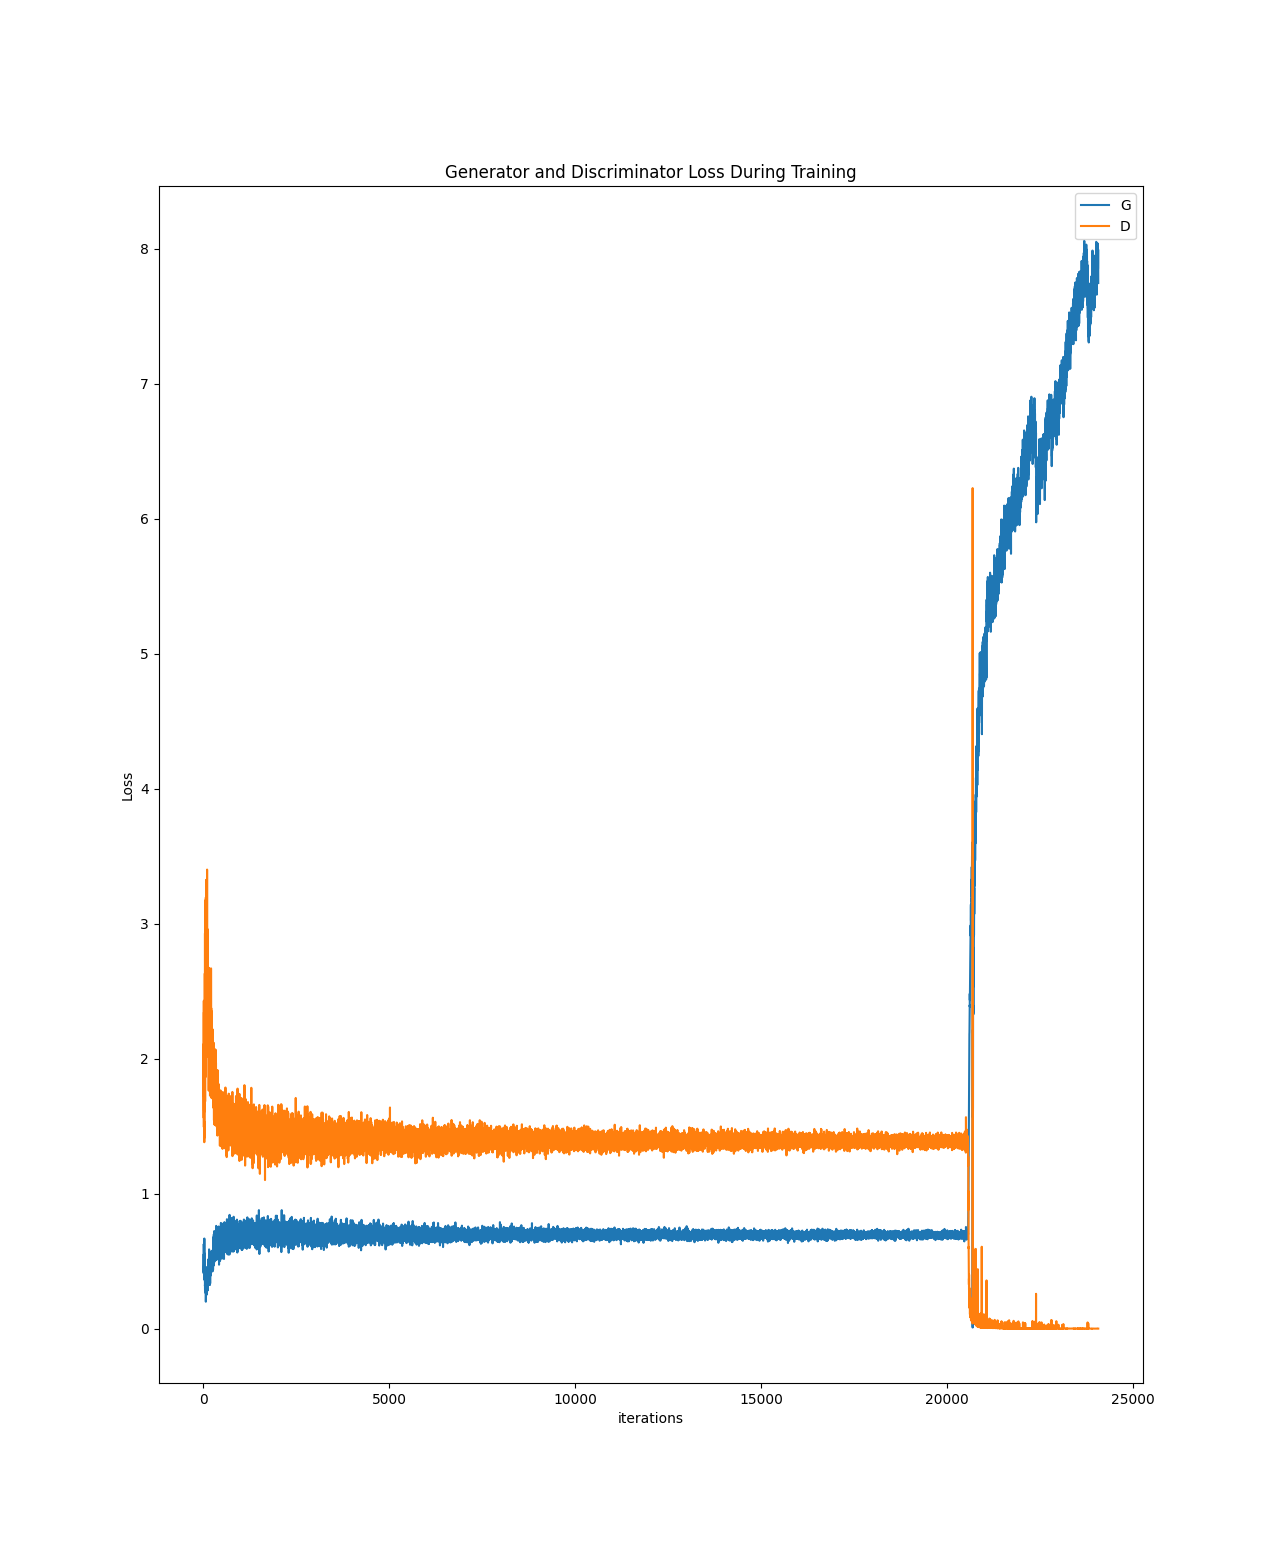
\includegraphics[width=0.9\textwidth, height=10cm]{GAN-loss-double_batch-Adam-no_random.png}
    \caption{%
        Loss of the GAN with double batching for the generator and no encoded
        random words for the discriminator.
    }\label{fig:ganLossAdamNoRandom}
\end{figure}

Here are some outputs of that model:

\begin{verbatim}
[0/10][0/6765]    Loss_D: 1.9186    Loss_G: 0.6208    D(x): 0.4685    D(G(z)): 0.5844 / 0.5884
shorter anything anything out go again out mary out prefer
machine shopping fish it's shopping prefer mistakes mistakes everything clear

[0/10][500/6765]    Loss_D: 1.4489    Loss_G: 0.7317    D(x): 0.5092    D(G(z)): 0.5200 / 0.4889
. ? of <PAD> <PAD> of of way she <PAD>
. ? of <PAD> <PAD> of of english she <PAD>

[0/10][1000/6765]    Loss_D: 1.5700    Loss_G: 0.6301    D(x): 0.4740    D(G(z)): 0.5423 / 0.5395
<PAD> untidy of <PAD> <PAD> <PAD> of way she <PAD>
<PAD> make of <PAD> <PAD> poor of way his <PAD>

...

[1/10][5200/6765]    Loss_D: 1.4087    Loss_G: 0.7026    D(x): 0.5035    D(G(z)): 0.5127 / 0.4960
<PAD> appropriated she she she <EOS> <EOS> <EOS> <PAD> <PAD>
<PAD> appropriated she she she <EOS> <EOS> <EOS> <EOS> <PAD>

[1/10][5700/6765]    Loss_D: 1.4143    Loss_G: 0.7011    D(x): 0.4879    D(G(z)): 0.5002 / 0.4968
worms <EOS> <PAD> ? why <PAD> <EOS> <EOS> <PAD> <PAD>
worms <EOS> worms <PAD> something <PAD> <PAD> <EOS> <PAD> <PAD>

[1/10][6200/6765]    Loss_D: 1.3873    Loss_G: 0.6957    D(x): 0.5044    D(G(z)): 0.5023 / 0.4997
? <EOS> do <PAD> you'll thing <EOS> <EOS> <PAD> <PAD>
? <EOS> do <PAD> of thing <EOS> <EOS> <EOS> <PAD>

\end{verbatim}

Here we seem to see that model has much harder time constructing actual
sentences. It puts \texttt{end-of-sequence}-tokens and padding at random places
and it hasn't really picked up on punctuation yet. But we are not yet at the
collapse seen in Figure~\ref{fig:ganLossAdamNoRandom}, so lets take a look at
some more outputs:

\begin{verbatim}
[2/10][1950/6765]    Loss_D: 1.3705    Loss_G: 0.7144    D(x): 0.5072    D(G(z)): 0.4975 / 0.4904
get appropriated of is <EOS> <EOS> <EOS> delayed <PAD> <PAD>
get appropriated of is <EOS> <EOS> <EOS> a <PAD> <PAD>

[2/10][2450/6765]    Loss_D: 1.3432    Loss_G: 0.6959    D(x): 0.5086    D(G(z)): 0.4853 / 0.4991
that criticisms of to that <EOS> <EOS> <EOS> <PAD> <PAD>
that criticisms of him <EOS> <EOS> <EOS> <EOS> <EOS> <PAD>

[2/10][2950/6765]    Loss_D: 1.4055    Loss_G: 0.6989    D(x): 0.4902    D(G(z)): 0.4984 / 0.4975
is much not to <EOS> <PAD> <PAD> <PAD> <PAD> <PAD>
is my not <EOS> <EOS> <PAD> <PAD> <PAD> <PAD> <PAD>

...

[3/10][200/6765]    Loss_D: 1.3366    Loss_G: 0.7089    D(x): 0.5265    D(G(z)): 0.4985 / 0.4929
. . . . <EOS> <EOS> <EOS> <PAD> <PAD> <PAD>
. . . . <EOS> <EOS> <EOS> <PAD> <PAD> <PAD>

[3/10][700/6765]    Loss_D: 0.0100    Loss_G: 5.0729    D(x): 0.9973    D(G(z)): 0.0073 / 0.0072
<PAD> <PAD> <PAD> <PAD> <PAD> <PAD> <PAD> <PAD> <PAD> <PAD>
<PAD> <PAD> <PAD> <PAD> <PAD> <PAD> <PAD> <PAD> <PAD> <PAD>

[3/10][2700/6765]    Loss_D: 0.0017    Loss_G: 6.7365    D(x): 0.9996    D(G(z)): 0.0013 / 0.0013
make make make make make make make make make make
make make make make make make make make make make

\end{verbatim}

Here it seems that the model was beginning to pick up on where to put
\texttt{end-of-sequence}-tokens and padding (though not to what extent) but when
the collapse happens, the generator completely stops working and just outputs
single-word sentences. The collapse is also clearly represented in both $D(x)$
and $D(G(z))$.

Finally, for comparison, lets look at some examples of the GAN model, when it is
trained on a TransformerModel that hasn't learned about padding and
\texttt{end-of-sequence}-tokens:

\begin{verbatim}
are thank new to you . suspicious suspicious suspicious prevents suspicious
mafia mafia mafia subtitled

something troll me watched watched . suspicious suspicious suspicious suspicious
mafia mafia mafia mafia mafia

your ignored delayed delayed . helpless helpless helpless helpless helpless
helpless suspicious helpless helpless helpless

it's , , him looking expect . . housewarming housewarming housewarming
suspicious mercury mercury mercury

for change but do i . suspicious suspicious suspicious suspicious suspicious
suspicious suspicious mafia mafia

i mohammed convenience play the . suspicious suspicious suspicious suspicious
suspicious mafia mafia mafia mafia

he used was donated money . subtitled suspicious suspicious suspicious
suspicious suspicious suspicious scientist scientist
\end{verbatim}

It is interesting note, that it seems to attempt generating a sentence with
different word and some kinds of sentence constructs, but after it outputs a
punctuation mark it almost just outputs the same word over and over. This
indicates that is has learned the concept of sentence length and some
consequence of an end of sequence marker (such as the punctuation mark).


\subsection{Further research and improvements}\label{sec:furtherResearch}
We believe that the full potential of using the TransformerModel encodings in a
GAN has yet to be revealed. Training a GAN without batching using a variable
input length with EOS tokens, could lead to further improvements. Another
approach to explore is using the original transformer encoder-decoder stack in
place of the two encoder stacks approach we used.

Furthermore using a fixed size encoding such as the RnnModel makes training the
encoder much harder but should make training the GAN much easier. As such
getting a good Teacher model using this approach could potentially lead to large
improvements in the GAN model. To this, it is also worth considering, that where
some encoders might just learn to map words to some hidden state, a better
encoder could probably inject syntax and sentence-meaning, which might also help
a GAN model perform better.

There might also be advantages in systematically testing how training evolves
with different optimizers, such as Adam, SGD, Adagrad, etc.\ and with different
learning rates. The GAN model is clearly very fragile and it seems that very
careful tuning of hyperparameters is needed to avoid a collapse. Maybe it would
even be beneficial with dynamic hyperparameters that adapts to the state of the
GAN.\

Further, it would also be beneficial to get a better metric for evaluating the
performance of the GAN.\ The loss and the output of the discriminator gives a
hint to how the network is doing, but often it does not directly relate to how
seemingly `good' sentences produced by the generator of the model.

\section{Conclusion}\label{sec:conclusion}
We have explored two different ways of encoding sentences --- one, using a small
Transformer encoder stack and a simple feed-forward decoding netowrk, and
another using and RNN-based encoder and a more involved attention-based decoder.
We achieved good results with the first, but the second one took extremely long
to converge and only got to sub-par results.

We did manage to construct a GAN model that produced sentences with some
resemblance to the distribution it was trying to estimate. Especially, it seemed
to be able to end sentences properly (with punctuation,
\texttt{end-of-sequence}-tokens and padding) and its sentence-constructs were
different from total randomness.

However, the GAN model (when trained with Adam as its optimization algorithm)
always seemed to collapse at some point during training, where the generator
would no longer be able to get a sentence past the discriminator. We tried
increasing the batch size for the generator and also to stop training the
discriminator on encoded random words, but this only alleviated the problem so
much. Also, we saw that not using encoded random words preserved the stability
of the model much longer, but it became significantly worse at producing just
seemingly meaningful sentence-constructs (especially in regards to
\texttt{end-of-sequence}-tokens and padding).

With SGD, the model would not collapse, but instead it tended towards producing
very short sentences with a very, very low non-sensical vocabulary.

In conclusion our models did not produce sentences that were of any meaning to a human.
Our results indicate that better hyperparameters and a different inner architecture could
result in a GAN with more meaningful output.

\newpage
\printbibliography%

\end{document}

